\chapter{FPGA Hardware Implementation}
\section{OEM Hardware}
InterStream 4322C\cite{21} 
is a 2 port 10Gbps Ethernet Packet Capture Network Adapter
using an FPGA.

\section{NetFPGA}

The setup guide page\cite{22}

The Git Repository\cite{23}
\begin{verbatim}
  git clone git::/github.com/NetFPGA/netfpga
\end{verbatim}

The 10G development board\cite{24}
\url{http://netfpga.org/site/#/systems/3netfpga-10g/details/}

\url{http://www.digilentinc.com/Products/Detail.cfm?NavPath=2,400,796&Prod=NETFPGA}

\section{FPGA}
VHDL Basics and FPGA Implementation course

\begin{center}
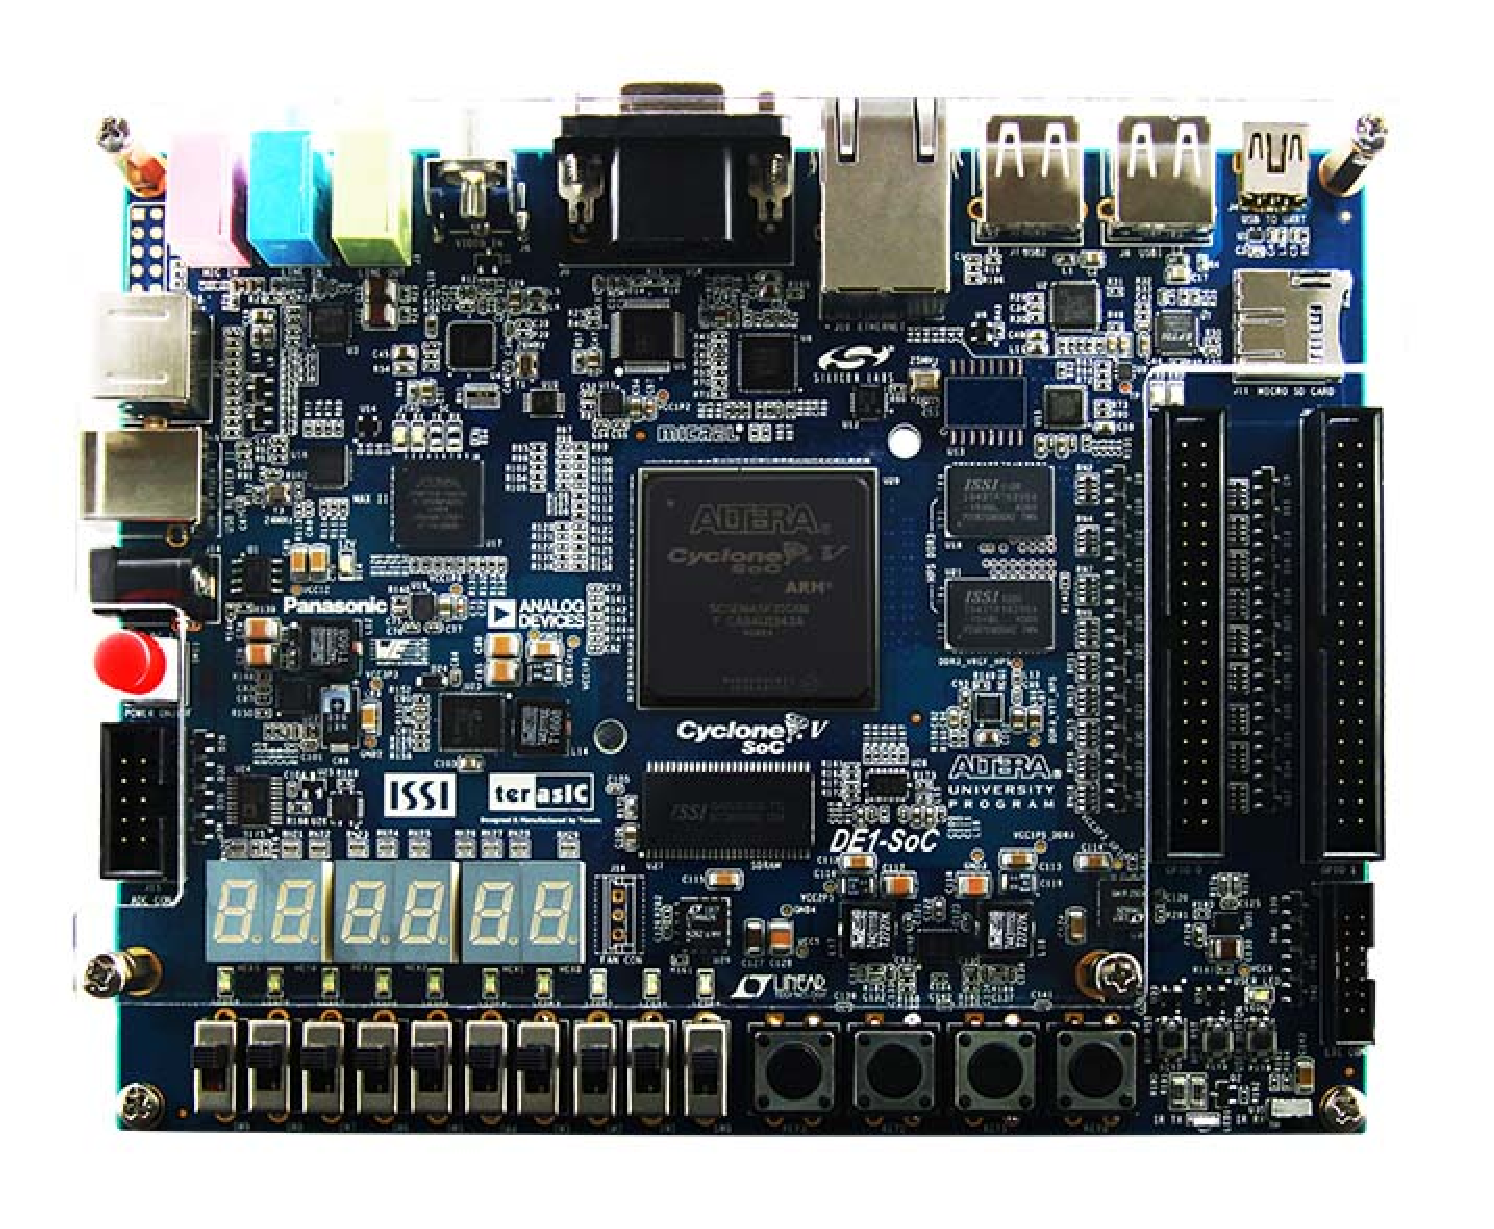
\includegraphics[scale=0.5]{eps/DE1SoC.eps}
\vskip 0.1in
\end{center}

\begin{center}
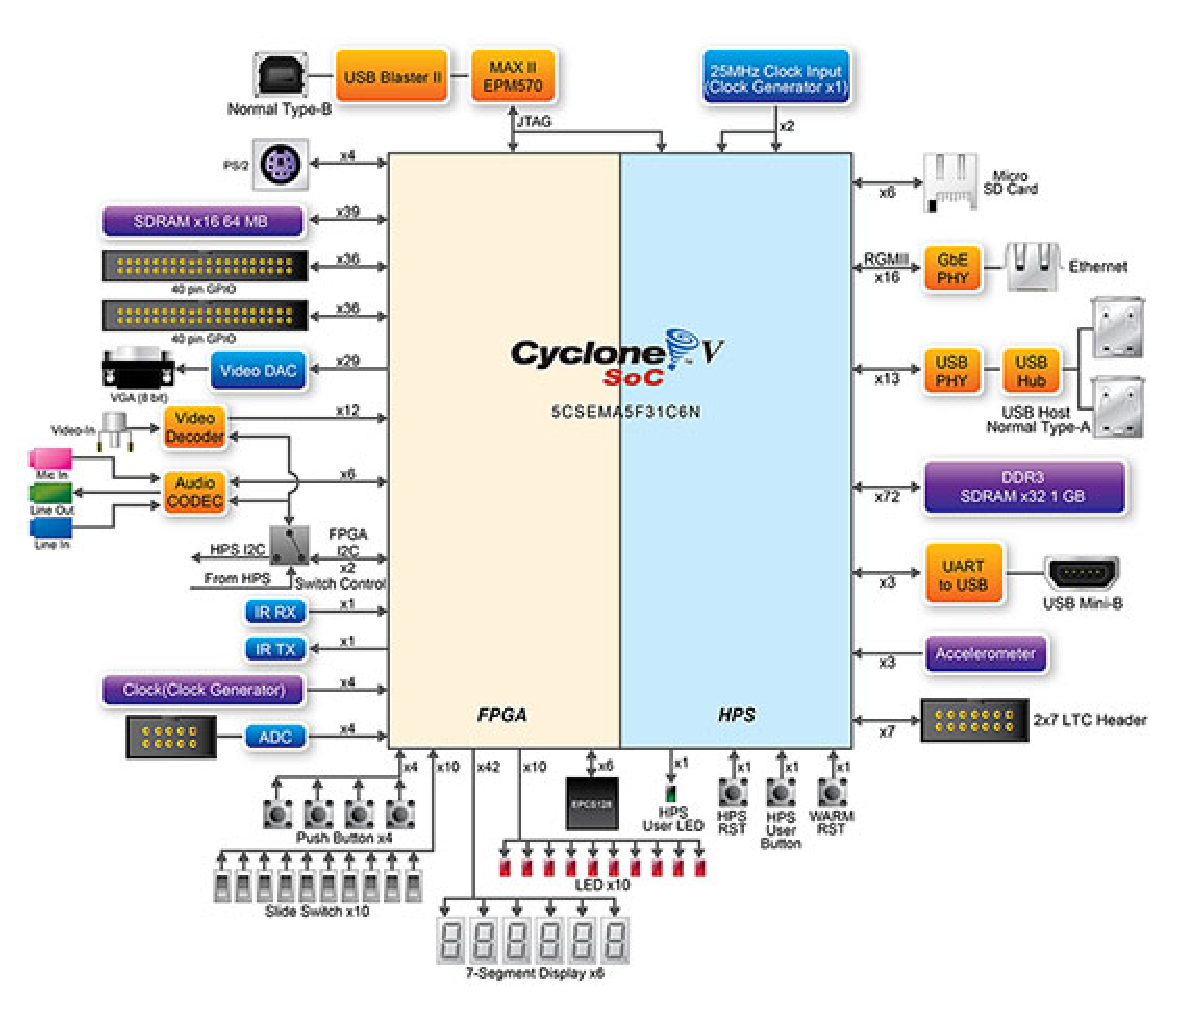
\includegraphics[scale=0.75]{eps/DE1SoCports.eps}
\vskip 0.1in
\end{center}

\section{FPGA Background}
\begin{itemize}
\item {\bf First Use}
\url{http://wl.altera.com/customertraining/webex/Begin_Simple_FPGA_Design/presentation.html}
\item Hardware-Based Packet Filtering Using FPGAs\cite{25}
\item Design of a Embedded Ethernet Packet Sniffer\cite{26}
\end{itemize}

\section{DE1-SoC Setup}
The Quartus II software package needs to be installed.

The DE1 board communicates using COM3 @ 115200/8/1 baud rate, no parity.

The board runs a linux operating system image from a micro-SD card.
The only login is root with no password.




\subsection{Hardware Tradeoff Matrix\cite{4}}
\begin{tabular}{llllll}
         &x86&GPU&DSP&FPGA&$\mu{}$C\\
embed   &maybe &hard      &easy      &easy&easy\\
low power&unusual &nope  &sometimes &sometimes &yes\\
float op&good&excellent&excellent&possible&nope\\
int op&excellent&excellent&excellent&excellent&mediocore\\
control flow&excellent&challenging&air&challenging&excellent\\
io&mediocore&nope&ok&ginormous&ok\\
pipelining&nope&nope&nope&yes&nope\\
programmable&easy&medium&medius&challenging&easy\\
timing control&medium&what?&fair&excellent&fair\\
\end{tabular}

state machines / random numbers 
PSHDL / myHDL / Verilog / VHDL

Xilinx / Altera / Actel (microsem) / Lattice

Ethernet hardware chip
news.thomasnet.com/fullstory/hardwired-tcp-ip-ic-offloads-stack-for-high-speed-internet-490029

\subsection{FPGA Development Boards\cite{4}}
\begin{tabular}{llll}
& actel&altera&xilinx\\
cheap&PSHDL board&DE0-Nano&Papilo One (Spartan 3)\\
&&bemicro CV&mojo Vs (spartan 6)\\
&&&XuLA2-LX25\\
powerful&igloo 2 boards&cyclone 5/arria&artix/kintex/virtex\\
SoC&smartfusion2 starter kit&EBV SoCrates&MicroZedBoard\\
&SmartFusion Starter kit&&parallella\\
CPU+FPGA&Daenkrake&&Logi\\
\end{tabular}

deny by default

disaster recovery


stealing backups
recovery plan

software
  user-mode
  kernel-mode
  hypervisor
  firmware
  microcode
  hardware
  physics

hardware exfilt:
  http://es.slideshare.net/ortegaalfredo/deep-submicronbackdoorsortegasyscan2014slides
    modify chip to detect sequence
    toggle hardware line (e.g. led) to generate radio freq
    listen with radio

infilltration

size of information

  key is easy... use blinds

  database is hard ... large volume

cloud?

sysadmin attacks (snowden/anthem)

fpga/asic

runtime reconfigurable systems

\url{http://media.ccc.de/browse/congress/2013/30C3_-_5443_-_en_-_saal_g_201312281830_-_introduction_to_processor_design_-_byterazor.html#video&t=370}

\url{http://byterazor.federationhq.de/download/handout_30C3.pdf}

fpga 50 dollars

  serial cable

  logic analyzer

  VHDL / Verilog

\url{http://tama-www.informatik.uni-hamburg.ed/vhdl/doc/cookbook/VHDL-Cookbook.pdf}

www.altera.com 6Gbps (starter kit)

regular, random machine audits (aka drug policy)

work from home?

Ring-level security policy?

finding out (e.g. watermarks, RFID tags)

dual computer policy? (plugged USB/secure only networking/loctite screws)

\begin{quote}
"Many businesses erro by putting too much faith in technology alone,
or by starting a security program with a technology blitz. The best
security technology in the world won't produce a good return on
investment without the foundation of security processes, policies, and
education. Instead, businesses should start by evaluating employee
behavior and the associated risks based on factors such as the locale
and the threat landscape. Then treat education, security training, and
business processes can be scuplted around that intelligence. At that
point, appropriate investments in security technology can be applied"
\cite{2}
\end{quote}

outsiders let inside

  "cleaner attacks"/"copier attacks"/"video stream encrypt"

BYOD

mobility

cloud

internet

wifi

USB

unauthorized software

email

provisioning

privileged account management

managing access

